% CVPR 2022 Paper Template
% based on the CVPR template provided by Ming-Ming Cheng (https://github.com/MCG-NKU/CVPR_Template)
% modified and extended by Stefan Roth (stefan.roth@NOSPAMtu-darmstadt.de)

\documentclass[10pt,twocolumn,letterpaper]{article}

%%%%%%%%% PAPER TYPE  - PLEASE UPDATE FOR FINAL VERSION %%%%%%%%%
%\usepackage[review]{cvpr}      % To produce the REVIEW version
%\usepackage{cvpr}              % To produce the CAMERA-READY version
\usepackage[pagenumbers]{cvpr} % To force page numbers, e.g. for an arXiv version

% Include other packages here, before hyperref.
\usepackage{graphicx}
\usepackage{amsmath}
\usepackage{amssymb}
\usepackage{booktabs}
\usepackage{float}
\usepackage{arydshln}
\usepackage{enumitem}


% It is strongly recommended to use hyperref, especially for the review version.
% hyperref with option pagebackref eases the reviewers' job.
% Please disable hyperref *only* if you encounter grave issues, e.g. with the
% file validation for the camera-ready version.
%
% If you comment hyperref and then uncomment it, you should delete
% ReviewTempalte.aux before re-running LaTeX.
% (Or just hit 'q' on the first LaTeX run, let it finish, and you
%  should be clear).
\usepackage[pagebackref,breaklinks,colorlinks]{hyperref}


% Support for easy cross-referencing
\usepackage[capitalize]{cleveref}
\crefname{section}{Sec.}{Secs.}
\Crefname{section}{Section}{Sections}
\Crefname{table}{Table}{Tables}
\crefname{table}{Tab.}{Tabs.}

\raggedbottom
\begin{document}

%%%%%%%%% TITLE - PLEASE UPDATE %%%%%%%%%
\title{DLP Lab3: MaskGIT for Image Inpainting}

\author{Yi-Hsiang Ho, 111550106
% For a paper whose authors are all at the same institution,
% omit the following lines up until the closing ``}''.
% Additional authors and addresses can be added with ``\and'',
% just like the second author.
% To save space, use either the email address or home page, not both
% \and
% Second Author\\
% Institution2\\
% First line of institution2 address\\
% {\tt\small secondauthor@i2.org}
}
\maketitle

%%%%%%%%% BODY TEXT %%%%%%%%%

% ------------------------- Introduction -------------------------

\section{Introduction}
\label{sec:intro}

In this lab, we implement the Masked Generative Image Transformer (MaskGIT)
for image inpainting. MaskGIT utilizes a bidirectional transformer and
non-autoregressive iterative decoding, enabling parallel token prediction for
faster and more coherent image synthesis compared to traditional sequential models.

We implement the following components:

\begin{itemize}[itemsep=0pt]
  \item Multi-Head Self-Attention: Developed the transformer module for global context capture.
  \item Stage 2 Training: Trained the transformer to predict masked image tokens.
  \item Iterative Decoding: Implemented inpainting logic with confidence-based sampling.
  \item Mask-Scheduling: Integrated dynamic scheduling to manage mask ratios across iterations.
\end{itemize}

Results were evaluated using the Fréchet Inception Distance (FID) to quantify
image quality and diversity.


% -------------------- Implementation Details --------------------

\section{Implementation Details}
\label{sec:impl}

\subsection{Multi-Head Self-Attention}
\label{subsec:mha}

The multi-head attention module uses the scaled dot-product mechanism to model
global relationships across 16 parallel heads. Input features are projected into
query, key, and value tensors, then split for head-wise computation. Attention
scores are computed as $\mathbf{Q}\mathbf{K}^T/\sqrt{d_k}$, and normalized via
$\text{softmax}$. Then multiply with $\mathbf{V}$. The resulting context vectors
are concatenated and passed through a final linear layer to restore the original
embedding dimension while integrating diverse spatial information.

The implementation is as follows:

\begin{figure}[H]
  \centering
  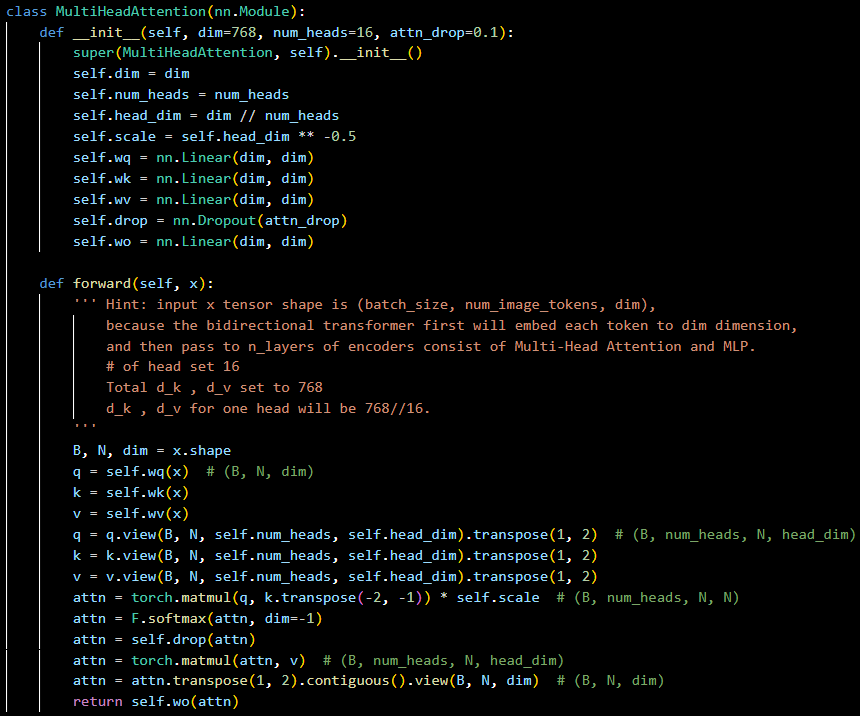
\includegraphics[width=\linewidth]{assets/impl-mha.png}
  \caption{\textbf{The implementation of multi-head attention}}
  \label{fig:impl-mha}
\end{figure}

\subsection{Stage 2 Training}

Stage 2 training focuses on optimizing the bidirectional transformer
through Masked Visual Token Modeling (MVTM). The input image is first
encoded into a $16 \times 16$ grid of discrete visual tokens using a pre-trained
and frozen VQGAN encoder (\cref{fig:impl-train-enc}). During each training step
(\cref{fig:impl-train-forward}), a masking ratio is sampled based on a cosine
scheduling function (\cref{fig:impl-train-gamma}), and a corresponding subset
of tokens is randomly replaced with a special mask token ID. In the forward
pass, these masked indices are fed into the bidirectional transformer to predict
the original visual tokens. The model is trained using cross-entropy loss between
the predicted logits and the ground-truth tokens, incorporating a label smoothing
of 0.1 to improve robustness and prevent over-confident predictions. Additionally, 
gradient accumulation is implemented to simulate a larger effective batch size, 
where gradients are normalized and accumulated over multiple mini-batches before 
applying gradient clipping and performing an optimization step.

\begin{figure}[H]
  \centering
  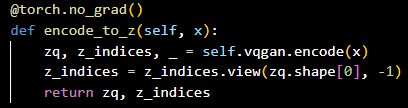
\includegraphics[width=\linewidth]{assets/impl-train-enc.png}
  \caption{\textbf{The implementation of Stage 2 Training (Fed into pretrained VQGAN encoder)}}
  \label{fig:impl-train-enc}
\end{figure}

\begin{figure}[H]
  \centering
  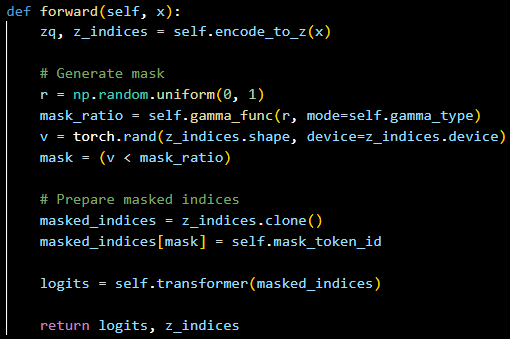
\includegraphics[width=\linewidth]{assets/impl-train-forward.png}
  \caption{\textbf{The implementation of Stage 2 Training (Forward pass)}}
  \label{fig:impl-train-forward}
\end{figure}

\begin{figure}[H]
  \centering
  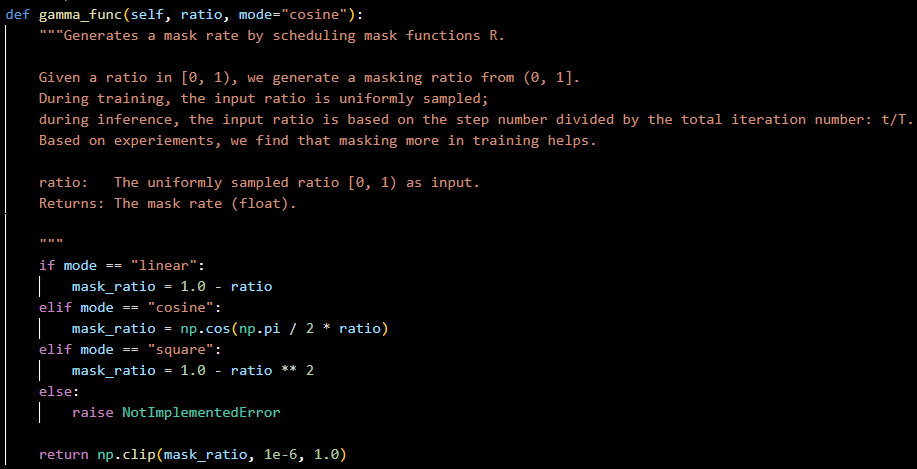
\includegraphics[width=\linewidth]{assets/impl-train-gamma.png}
  \caption{\textbf{The implementation of Stage 2 Training (Gamma function)}}
  \label{fig:impl-train-gamma}
\end{figure}

\begin{figure}[H]
  \centering
  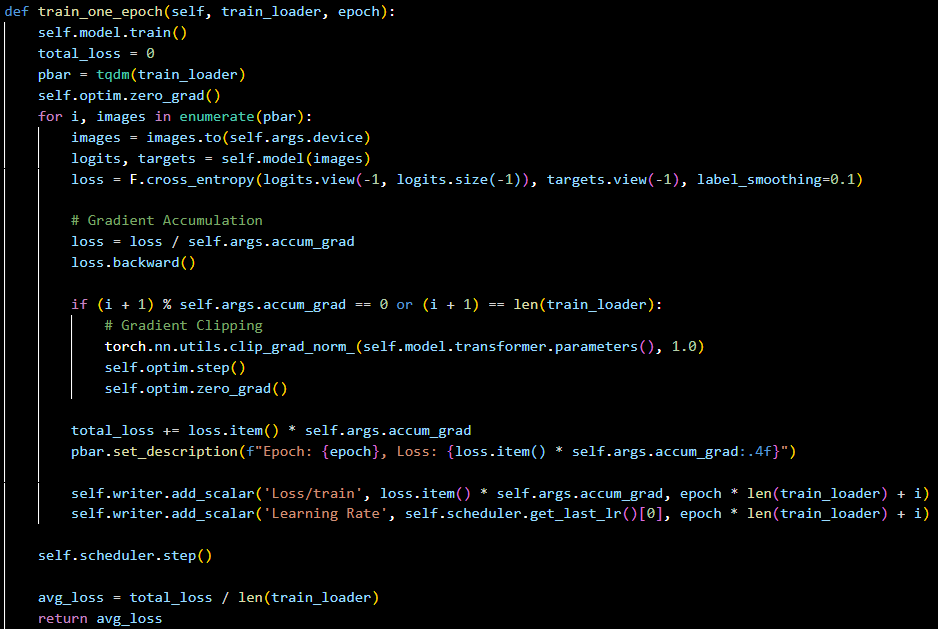
\includegraphics[width=\linewidth]{assets/impl-train-train-1-step.png}
  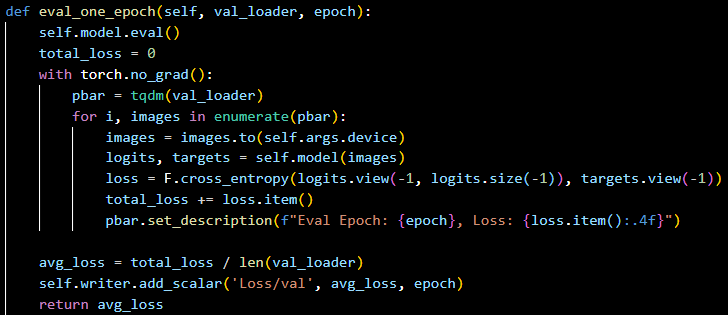
\includegraphics[width=\linewidth]{assets/impl-train-eval.png}
  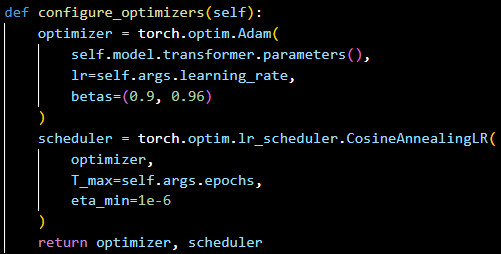
\includegraphics[width=\linewidth]{assets/impl-train-optim.png}
  \caption{\textbf{The implementation of Stage 2 Training (Training)}}
  \label{fig:impl-train-train}
\end{figure}

\begin{figure}[H]
  \centering
  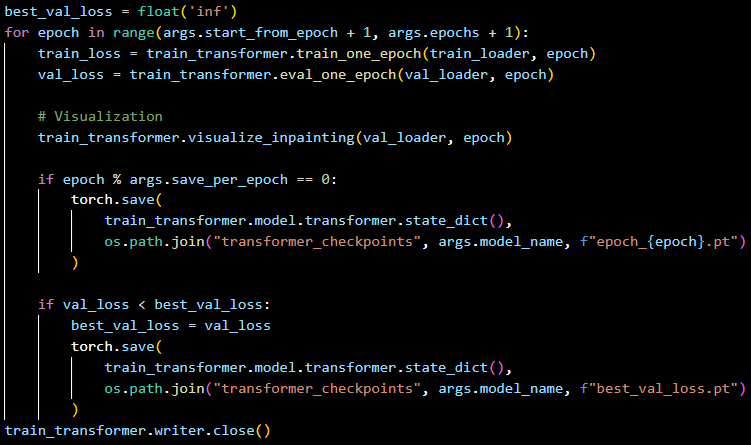
\includegraphics[width=\linewidth]{assets/impl-train-train-whole.png}
  \caption{\textbf{The implementation of Stage 2 Training (Training loop)}}
  \label{fig:impl-train-train-whole}
\end{figure}

\subsection{Inference}

The inference process in MaskGIT employs a non-autoregressive iterative decoding
strategy to reconstruct the masked regions of an image. Starting from an initial
set of masked visual tokens, the model performs a fixed number of decoding
iterations $T$. In each iteration, the bidirectional transformer predicts the
probability distributions for all masked positions in parallel. For each
position, a token is sampled from the distribution, and a confidence score is
assigned based on its prediction probability. To introduce diversity, temperature
annealing and Gumbel noise are incorporated into the confidence calculation. A
mask scheduling function $\gamma(t/T)$ determines the number of tokens to remain
masked in the next step, where tokens with the lowest confidence scores are
re-masked. This iterative refinement allows the model to progressively generate a
coherent and high-quality image by focusing on the most certain regions first.

The implementation of the iterative decoding logic is shown below:

\begin{figure}[H]
  \centering
  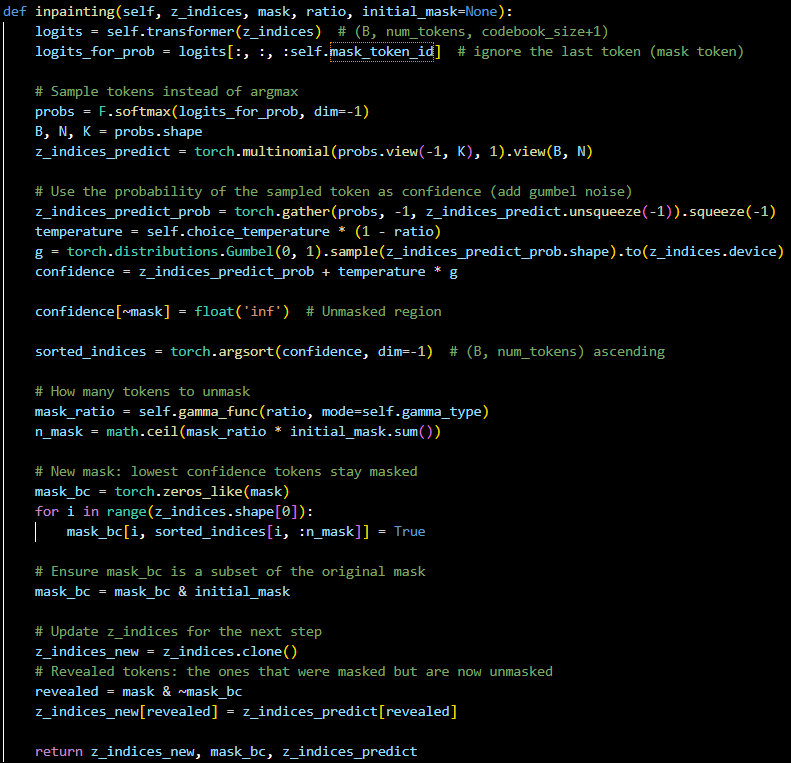
\includegraphics[width=\linewidth]{assets/impl-inpaint-1-step.png}
  \caption{\textbf{The implementation of iterative decoding for inference (1 step)}}
  \label{fig:impl-inpaint-1-step}
\end{figure}

\begin{figure}[H]
  \centering
  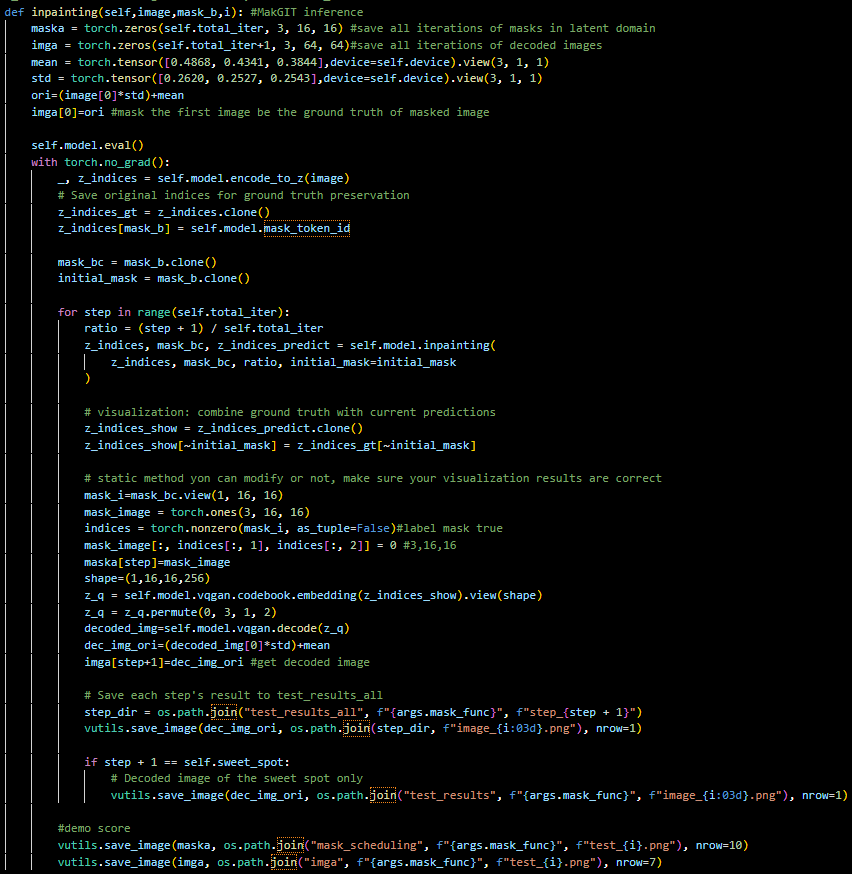
\includegraphics[width=\linewidth]{assets/impl-inpaint.png}
  \caption{\textbf{The implementation of iterative decoding for inference (inpaint loop)}}
  \label{fig:impl-inpaint}
\end{figure}

% ---------------------- Experimental Score ----------------------

\section{Experimental Score}

\subsection{Settings}
\label{subsec:settings}

\begin{table}[H]
  \centering
  \begin{tabular}{ll}
    \hline
    Setting & Value \\
    \hline
    Learning rate & $10^{-4}$ \\
    Epochs & $200$ \\
    Optimizer & Adam ($\beta_1=0.9, \beta_2=0.96$) \\
    Scheduler & Cosine annealing \\
    Batch size & $16$ \\
    Gradient accum. steps & $10$ \\
    Gradient clipping thres. & $1.0$ \\
    Label smoothing & $0.1$ \\
    \hline
  \end{tabular}
\end{table}

\subsection{Iterative Decoding}
\label{subsec:iter_dec}

The iterative decoding process is visualized in \cref{fig:exp-iterdec-latent}
and \cref{fig:exp-iterdec-img}. As shown in the figures, linear mode reduces
mask region linearly, while concave funcion (cosine, square-root) reduces mask
region slowly at the beginning and quickly at the end.

\begin{figure}[H]
  \centering
  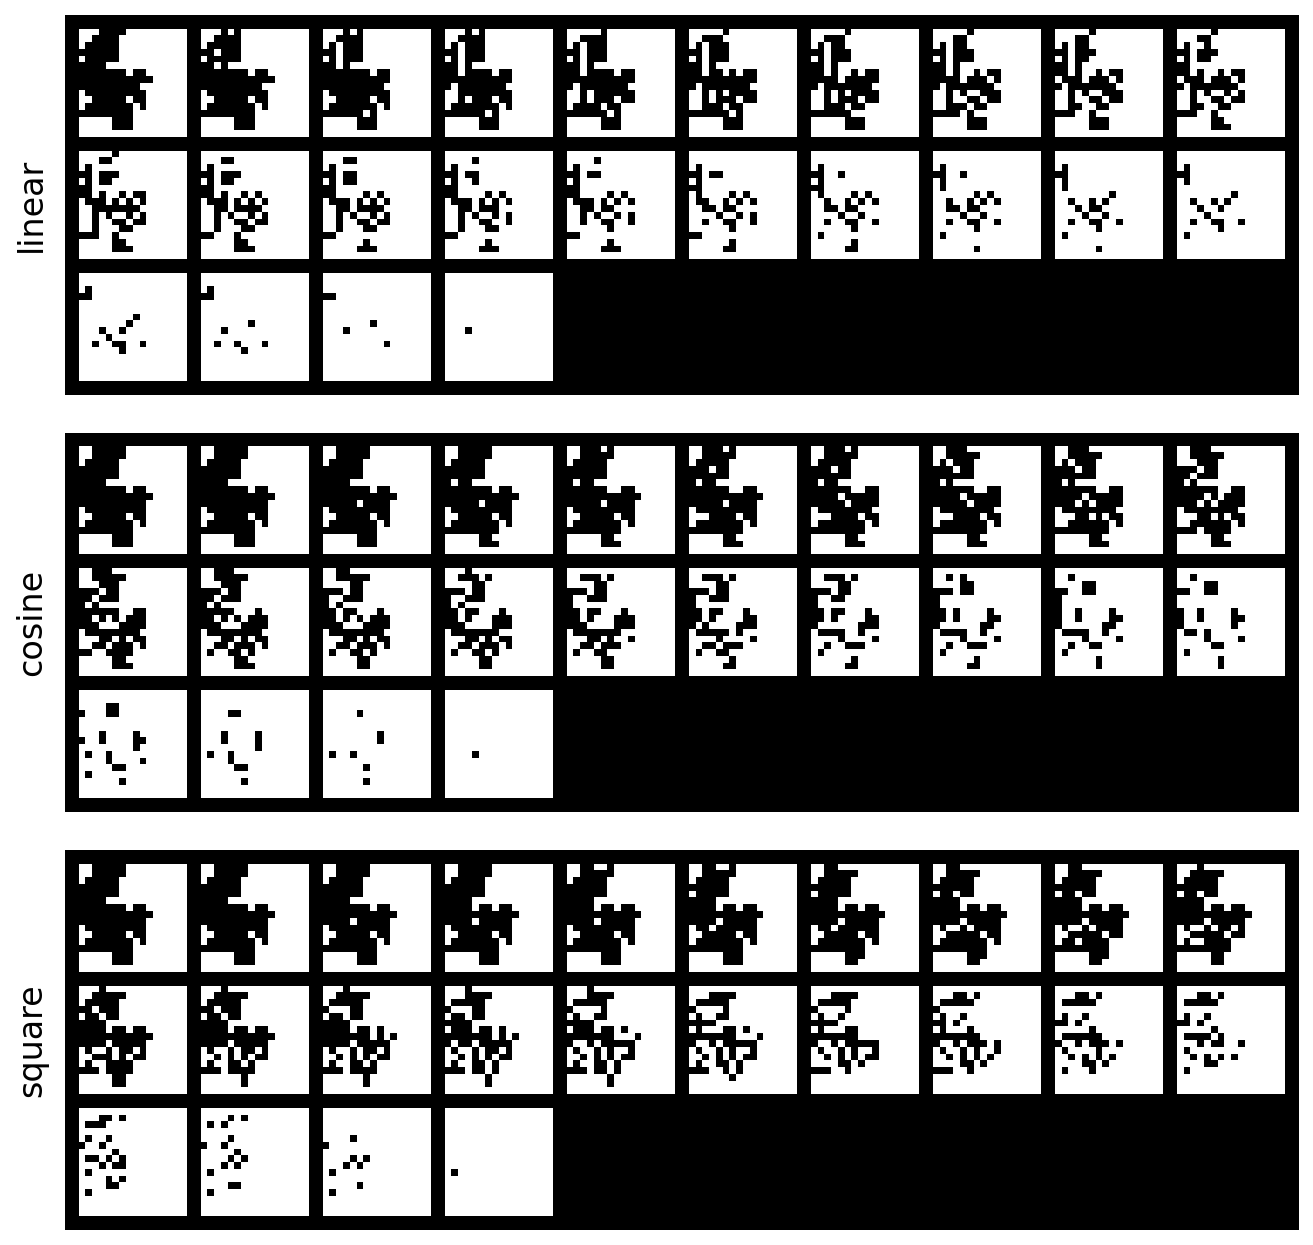
\includegraphics[width=\linewidth]{assets/exp-iterdec-latent.png}
  \caption{\textbf{Visualization of iterative decoding in latent space}}
  \label{fig:exp-iterdec-latent}
\end{figure}

\begin{figure}[H]
  \centering
  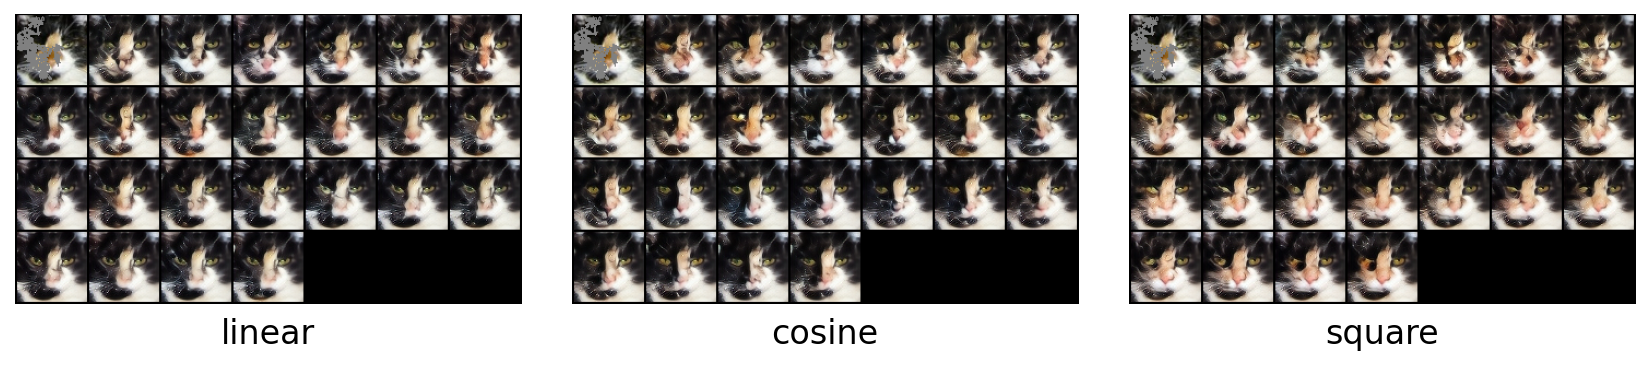
\includegraphics[width=\linewidth]{assets/exp-iterdec-img.png}
  \caption{\textbf{Visualization of iterative decoding in pixel space}}
  \label{fig:exp-iterdec-img}
\end{figure}

\subsection{FID Score}

The model's performance was evaluated using the FID. My best FID score is 29.1414, 
as shown in \cref{fig:exp-fid}. I also compared various mask scheduling functions, 
as shown in \cref{fig:exp-fid-compare}, where the cosine schedule consistently 
achieved the best results. The visual results of the best model are shown in
\cref{fig:exp-vis}.

\begin{figure}[H]
  \centering
  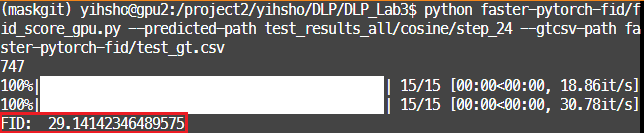
\includegraphics[width=\linewidth]{assets/exp-fid-screenshot.png}
  \caption{\textbf{Screenshot of best FID score}}
  \label{fig:exp-fid}
\end{figure}

\begin{figure}[H]
  \centering
  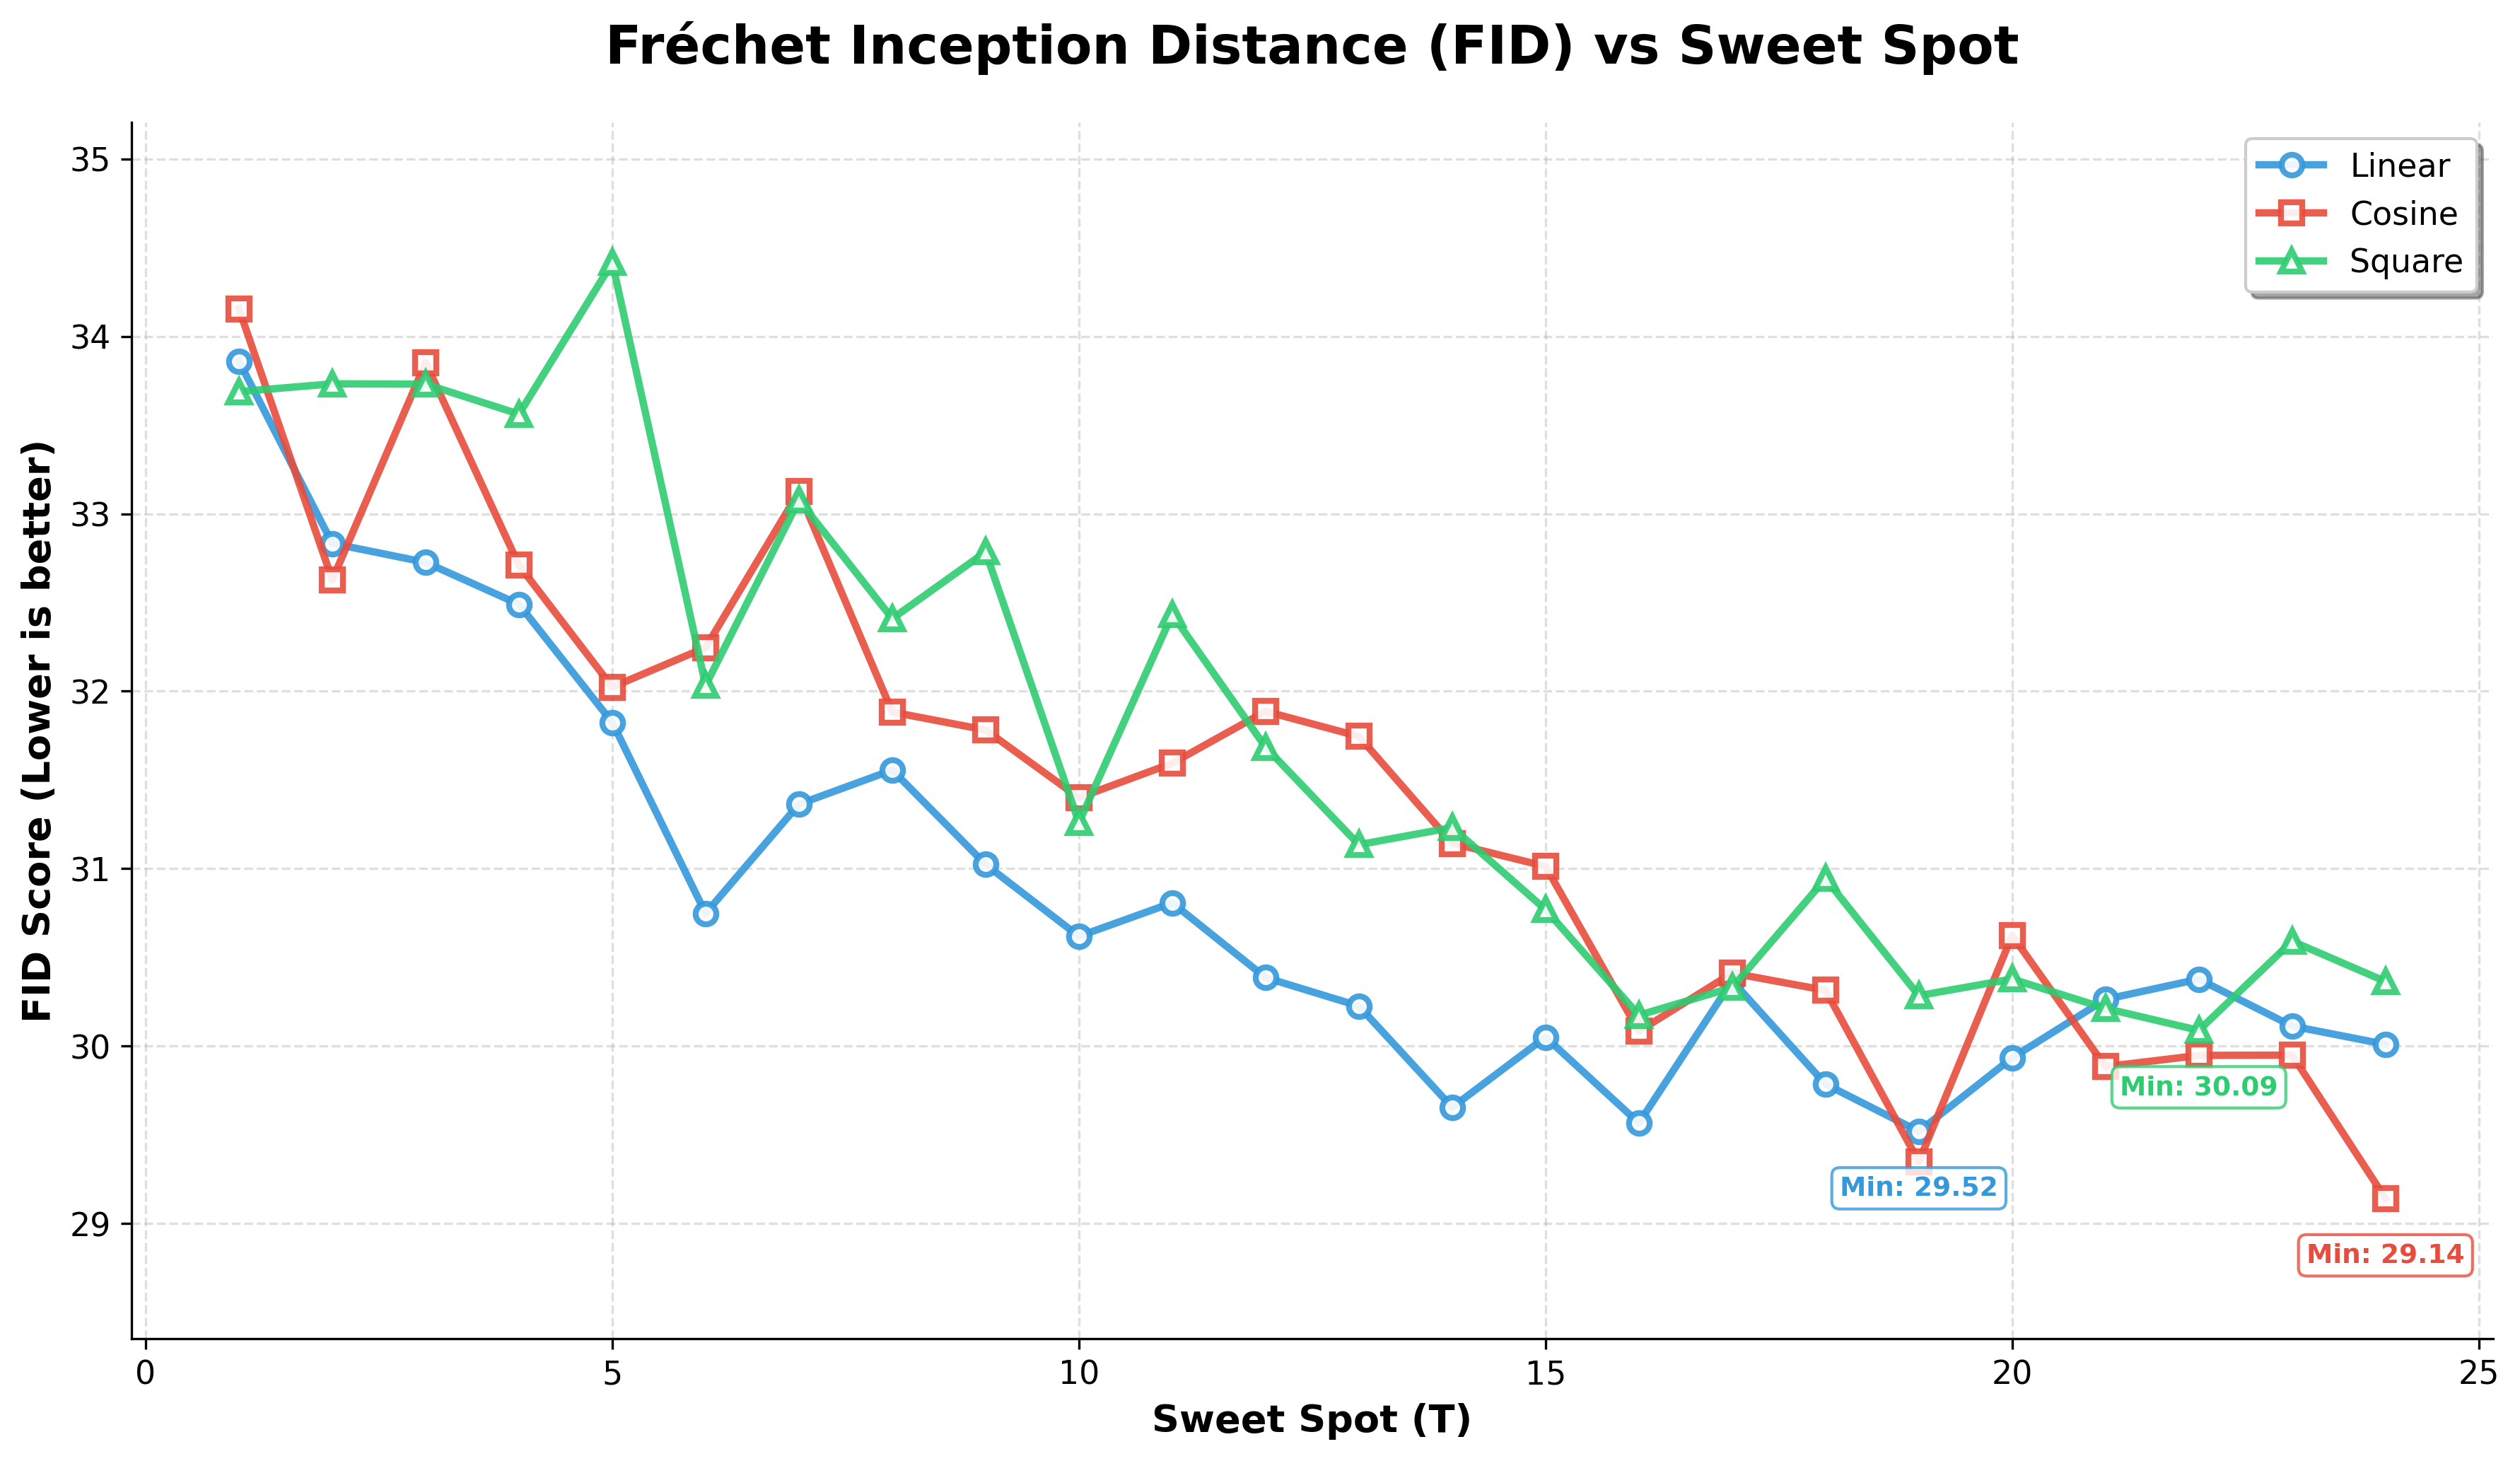
\includegraphics[width=\linewidth]{assets/exp-fid-comp.png}
  \caption{\textbf{FID score comparison across different mask functions}}
  \label{fig:exp-fid-compare}
\end{figure}

\begin{figure}[H]
  \centering
  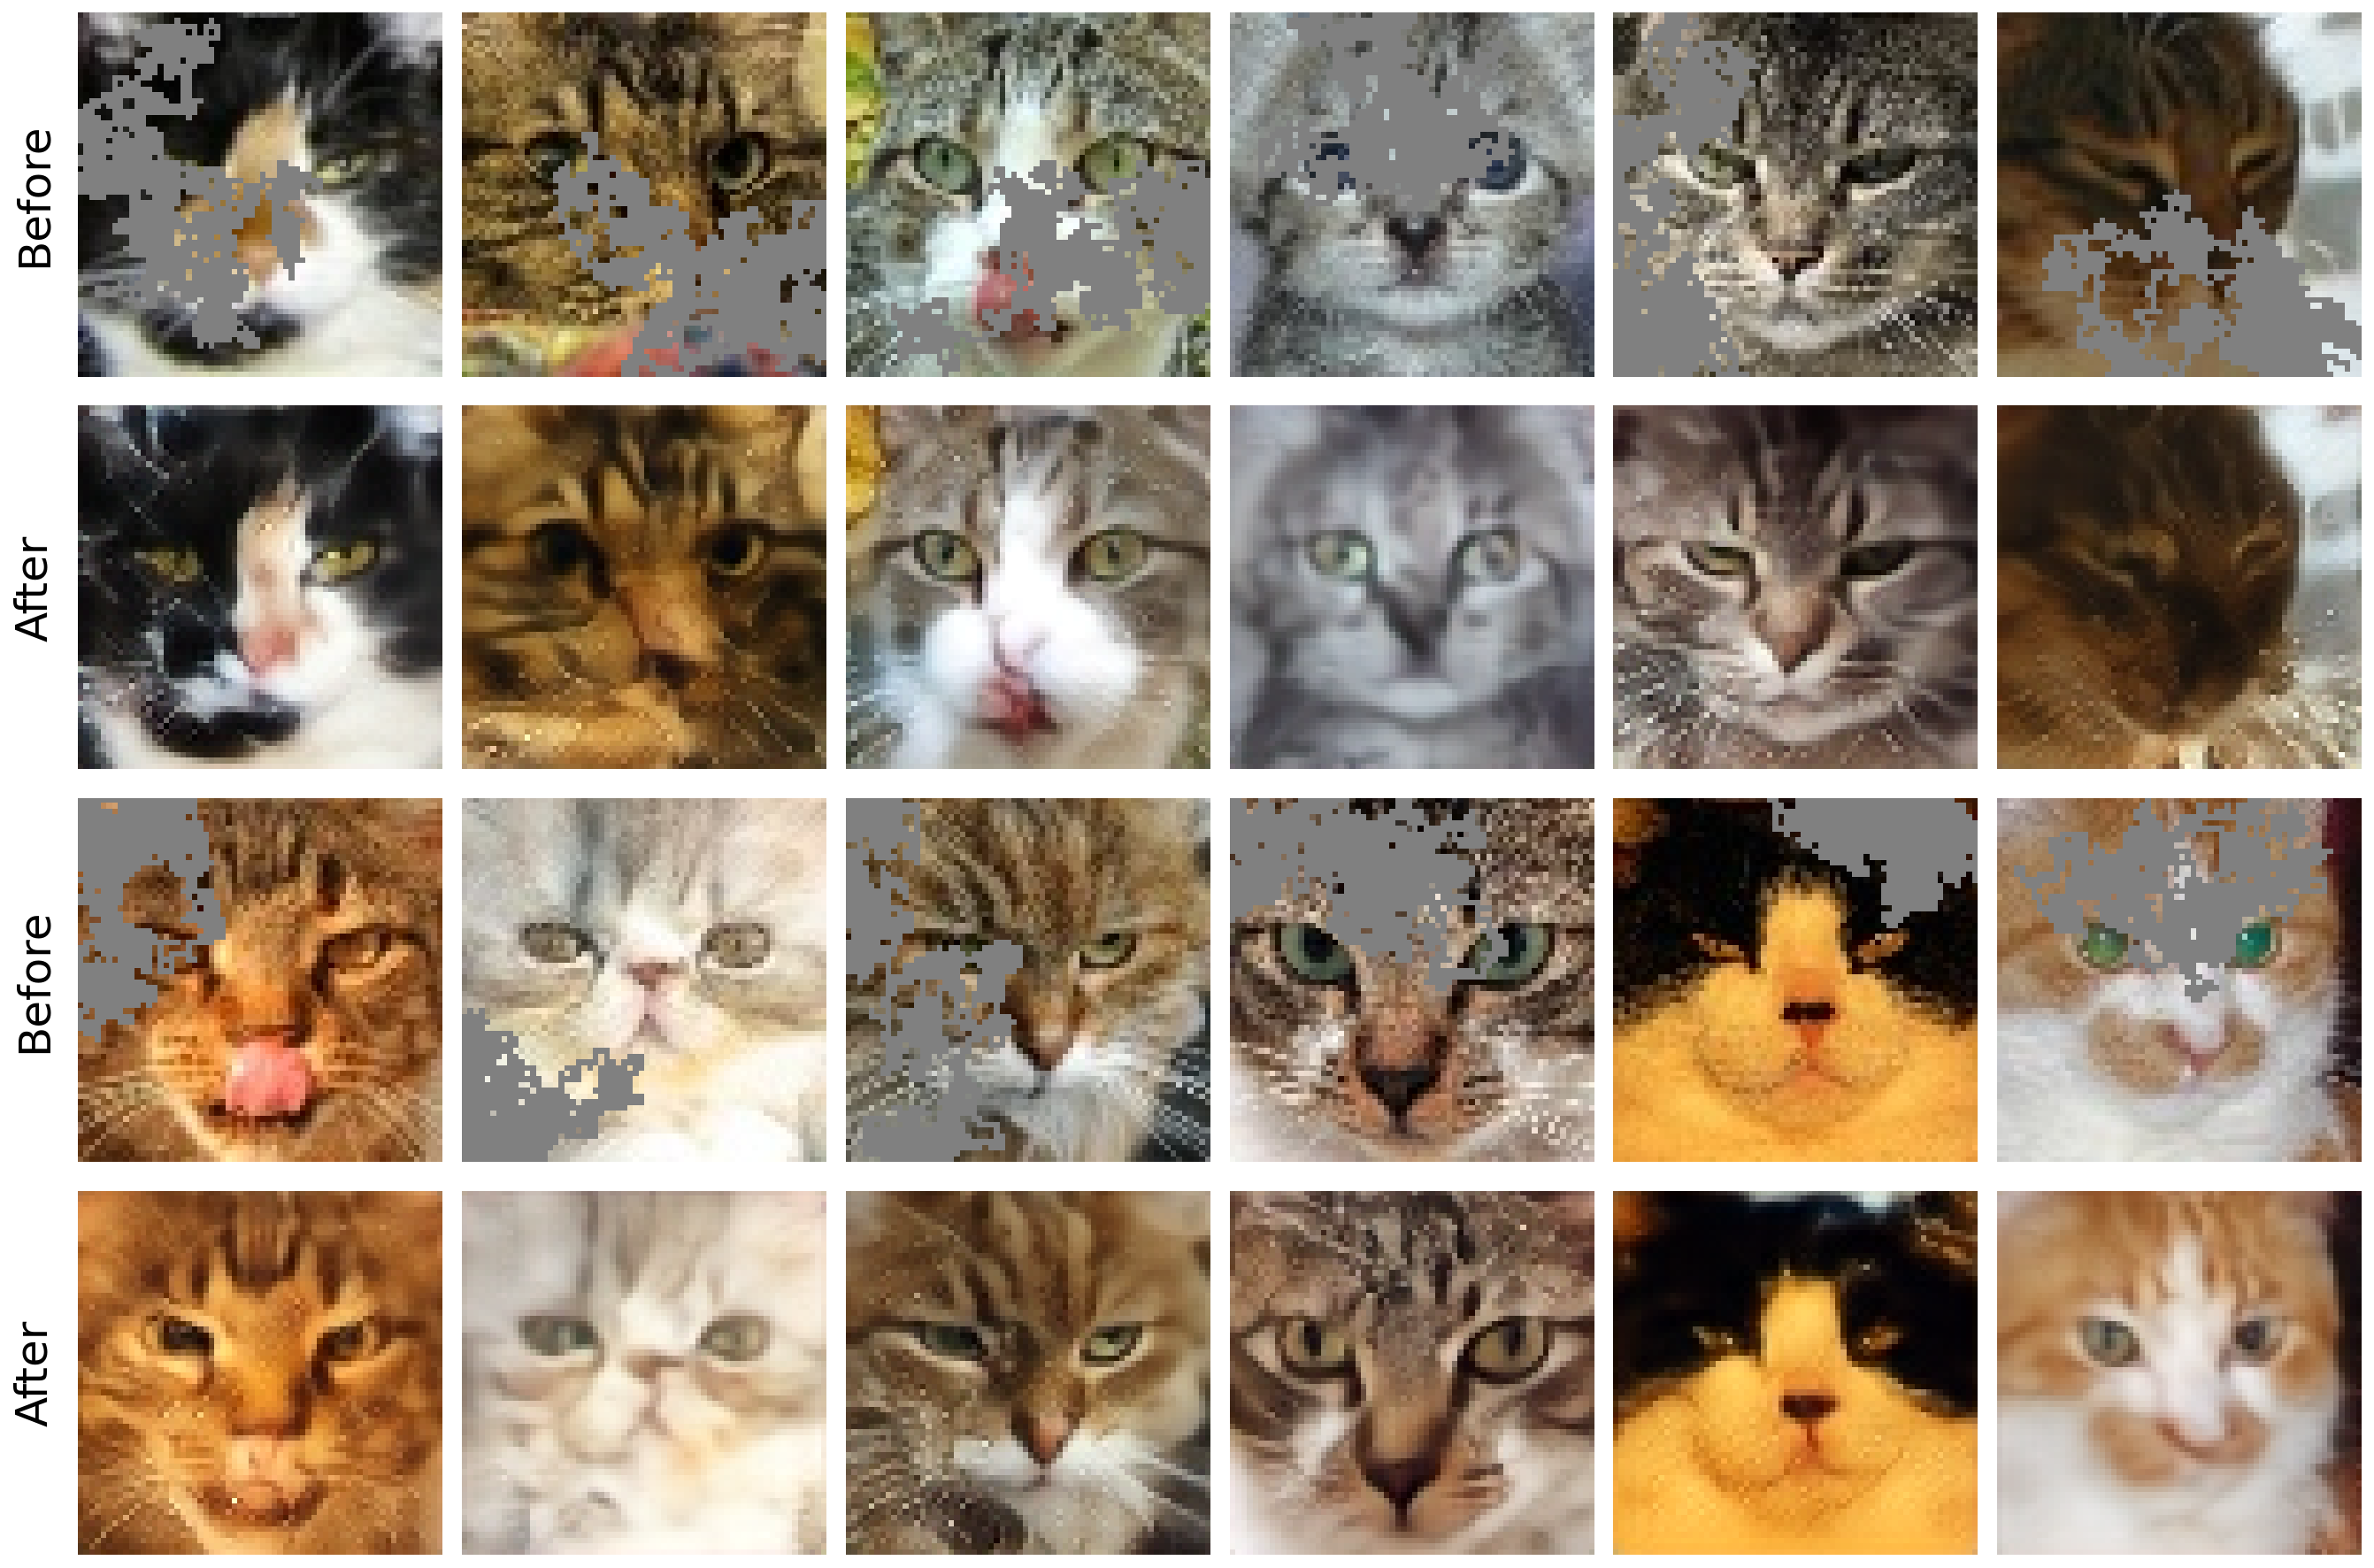
\includegraphics[width=\linewidth]{assets/exp-vis.png}
  \caption{\textbf{Generated images}}
  \label{fig:exp-vis}
\end{figure}

% -------------------------- Discussion --------------------------

\section{Discussion}
\label{sec:discussion}

\subsection{Sampling vs. \textbf{\texttt{argmax}}}
Although the initial skeleton code used \texttt{argmax} to select tokens, the 
original MaskGIT paper recommends sampling from the probability distribution. 
In my experiments, switching to stochastic sampling led to a better 
FID score.

\subsection{Gradient Accumulation}
Training transformers is often sensitive to batch size. However, GPU memory limits
restricted the batch size to 16. By implementing gradient accumulation over 10
steps, I effectively simulated a batch size of 160. This larger effective batch
size provided more stable gradient estimates during Stage 2 training, which led
to smoother convergence and a noticeable improvement in the final FID score.

% %%%%%%%%% REFERENCES %%%%%%%%%
% {\small
% \bibliographystyle{ieee_fullname}
% \bibliography{egbib}
% }

\end{document}